\chapter{Recognizing and Exploiting Personality Traits}
Real locks have a wide range of mechanical features and defects that help and hinder lock
picking. If a lock doesn't respond to scrubbing, then it probably has one of the traits
discussed in this chapter. To open the lock, you must diagnose the trait and apply the
recommended technique. The exercises will help you develop the mechanical sensitivity and
dexterity necessary to recognize and exploit the different traits.

\section{Which Way To Turn}
It can be very frustrating to spend a long time picking a lock and then discover that you
turned the plug the wrong way. If you turn a plug the wrong way it will rotate freely until it
hits a stop, or until it rotates 180 degrees and the drivers enter the keyway (see section 9.11).
Section 9.11 also explains how to turn the plug more than 180 degrees if that is necessary
to fully retract the bolt. When the plug is turned in the correct direction, you should feel
an extra resistance when the plug cam engages the bolt spring.

The direction to turn the plug depends on the bolt mechanism, not on the lock, but here
are some general rules. Cheap padlocks will open if the plug is turned in either direction, so
you can chose the direction which is best for the torque wrench. All padlocks made by the
Master company can be opened in either direction. Padlocks made by Yale will only open if
the plug is turned clockwise. The double plug Yale cylinder locks generally open by turning
the bottom of the keyway (i.e., the flat edge of the key) away from the nearest doorframe.
Single plug cylinder locks also follow this rule. See Figure 9.1. Locks built into the doorknob
usually open clockwise. Desk and filing cabinet locks also tend to open clockwise.

When you encounter a new kind of lock mechanism, try turning the plug in both directions. In the correct direction, the plug will be stopped by the pins, so the stop will feel
mushy when you use heavy torque. In the wrong direction the plug will be stopped by a
metal tab, so the stop will feel solid.

\begin{figure}
    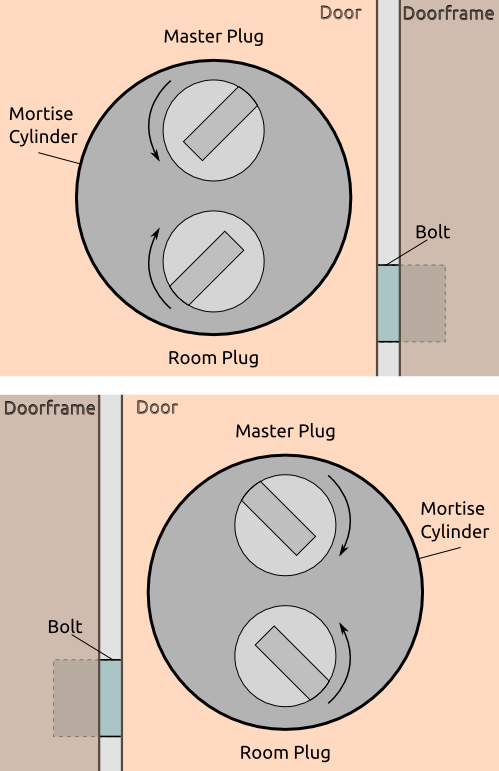
\includegraphics[scale=0.5]{figure9.1}
    \caption{Direction to turn plug}
\end{figure}

\section{How Far to Turn}
The companion question to which way to turn a lock is how far to turn it. Desk and filing
cabinet locks generally open with less than a quarter turn (90 degrees) of the plug. When
opening a desk lock try to avoid having the plug lock in the open position. Locks built into
doorknobs also tend to open with less than a quarter turn. Locks which are separate from
the doorknob tend to require a half turn to open. Deadbolt lock mechanisms can require
almost a full turn to open.

Turning a lock more than 180 degrees is a difficult because the drivers enter the bottom
of the keyway. See section 9.11.

\section{Gravity}
Picking a lock that has the springs at the top is different than picking one with the springs
at the bottom. It should be obvious how to tell the two apart. The nice feature of a lock
with the springs at the bottom is that gravity holds the key pins down once they set. With
the set pins out of the way, it is easy to find and manipulate the remaining unset pins. It is
also straight forward to test for the slight give of a correctly set pin. When the springs are
on top, gravity will pull the key pins down after the driver pin catches at the sheer line. In
this case, you can identify the set pins by noticing that the key pin is easy to lift and that it
does not feel springy. Set pins also rattle as you draw the pick over them because they are
not being pushed down by the driver pin.

\section{Pins Not Setting}
If you scrub a lock and pins are not setting even when you vary the torque, then some pin
has false set and it is keeping the rest of the pins from setting. Consider a lock whose pins
prefer to set from back to front. If the backmost pin false sets high or low (see Figure 9.2),
then the plug cannot rotate enough to allow the other pins to bind. It is hard to recognize
that a back pin has false set because the springiness of the front pins makes it hard to sense
the small give of a correctly set back pin. The main symptom of this situation is that the
other pins will not set unless a very large torque is applied.

When you encounter this situation, release the torque and start over by concentrating
on the back pins. Try a light torque and moderate pressure, or heavy torque and heavy
pressure. Try to feel for the click that happens when a pin reaches the sheer line and the
plug rotates slightly. The click will be easier to feel if you use a stiff torque wrench.

\section{Elastic Deformation}
The interesting events of lock picking happen over distances measured in thousandths of an
inch. Over such short distances, metals behave like springs. Very little force is necessary to deflect a piece metal over those distances, and when the force is removed, the metal will
spring back to its original position.

Deformation can be used to your advantage if you want to force several pins to bind at
once. For example, picking a lock with pins that prefer to set from front to back is slow
because the pins set one at a time. This is particularly true if you only apply pressure as
the pick is drawn out of the lock. Each pass of the pick will only set the frontmost pin that
is binding. Numerous passes are required to set all the pins. If the preference for setting is
not very strong (i.e., the axis of the plug holes is only slightly skewed from the plug's center
line), then you can cause additional pins to bind by applying extra torque. Basically, the
torque puts a twist in the plug that causes the front of the plug to be deflected further than
the back of the plug. With light torque, the back of the plug stays in its initial position, but
with medium to heavy torque, the front pin columns bend enough to allow the back of the
plug to rotate and thus cause the back pins to bind. With the extra torque, a single stroke
of the pick can set several pins, and the lock can be opened quickly. Too much torque causes
its own problems.

When the torque is large, the front pins and plug holes can be deformed enough to prevent
the pins from setting correctly. In particular, the first pin tends to false set low. Figure 9.2
shows how excess torque can deform the bottom of the driver pin and prevent the key pin
from reaching the sheer line. This situation can be recognized by the lack of give in the
first pin. Correctly set pins feel springy if they are pressed down slightly. A falsely set pin
lacks this springiness. The solution is to press down hard on the first pin. You may want to
reduce the torque slightly, but if you reduce torque too much then other pins will unset as
the first pin is being depressed.

It is also possible to deform the top of the key pin. The key pin is scissored between the
plug and the hull and stays fixed. When this happens, the pin is said to be false set high.

\section{Loose Plug }
The plug is held into the hull by being wider at the front and by having a cam on the back
that is bigger than the hole drilled into the hull. If the cam is not properly installed, the
plug can move in and out of the lock slightly. On the outward stroke of the pick, the plug
will move forward, and if you apply pressure on the inward stroke, the plug will be pushed
back.

The problem with a loose plug is that the driver pins tend to set on the back of the plug
holes rather than on the sides of the holes. When you push the plug in, the drivers will
unset. You can use this defect to your advantage by only applying pressure on the outward
or inward stroke of the pick. Alternatively, you can use your finger or torque wrench to
prevent the plug from moving forward.

\begin{figure}
    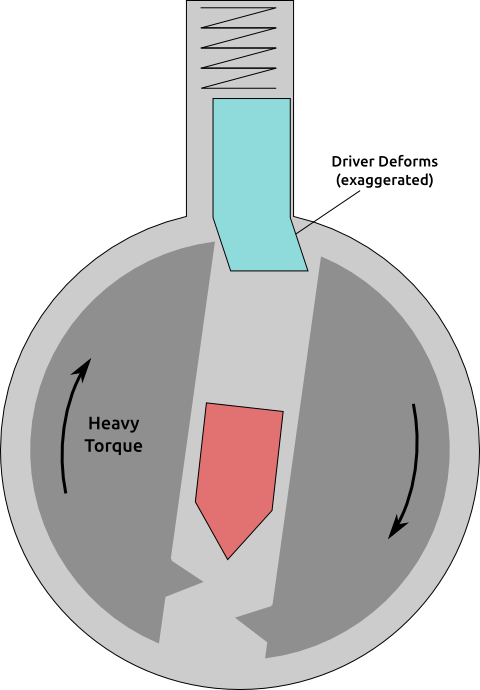
\includegraphics[scale=0.6]{figure9.2}
    \caption{Driver pin false set by elastic deformation}
\end{figure}

\section{Pin Diameter}
When the pair of pins in a particular column have different diameters, that column will react
strangely to the pressure of the pick.

The top half of Figure 9.3 shows a pin column with a driver pin that has a larger diameter
than the key pin. As the pins are lifted, the picking pressure is resisted by the binding friction
and the spring force. Once the driver clears the sheer line, the plug rotates (until some other
pin binds) and the only resistance to motion is the spring force. If the key pin is small enough
and the plug did not rotate very far, the key pin can enter the hull without colliding with
the edge of the hull. Some other pin is binding, so again the only resistance to motion is the
spring force. This relationship is graphed in the bottom half of the Figure. Basically, the
pins feel normal at first, but then the lock clicks and the pin becomes springy. The narrow
key pin can be pushed all the way into the hull without loosing its springiness, but when the
picking pressure is released, the key pin will fall back to its initial position while the large
driver catches on the edge of the plug hole.

The problem with a large driver pin is that the key pin tends to get stuck in the hull
when some other pin sets. Imagine that a neighboring pin sets and the plug rotates enough
to bind the narrow key pin. If the pick was pressing down on the narrow key pin at the same
time as it was pressing down on the pin that set, then the narrow key pin will be in the hull
and it will get stuck there when the plug rotates.

The behavior of a large key pin is left as an exercise for the reader.

\section{Beveled Holes and Rounded pins}
Some lock manufacturers (e.g., Yale) bevel the edges of the plug holes and/or round off
the ends of the key pins. This tends to reduce the wear on the lock and it can both help
and hinder lock picking. You can recognize a lock with these features by the large give in
set pins. See Figure 9.4. That is, the distance between the height at which the driver pin
catches on the edge of the plug hole and the height at which the key pin hits the hull is larger
(sometimes as large as a sixteenth of an inch) when the plug holes are beveled or the pins
are rounded. While the key pin is moving between those two heights, the only resistance to
motion will be the force of the spring. There won't be any binding friction. This corresponds
to the dip in the force graph shown in Figure 5.5.

A lock with beveled plug holes requires more scrubbing to open than a lock without
beveled holes because the driver pins set on the bevel instead of setting on the top of the
plug. The plug will not turn if one of the drivers is caught on a bevel. The key pin must
be scrubbed again to push the driver pin up and off the bevel. The left driver pin in Figure
9.6a is set. The driver is resting on the bevel, and the bottom plate has moved enough to
allow the right driver to bind. Figure 9.6b shows what happens after the right driver pin
sets. The bottom plate slides further to the right and now the left driver pin is scissored
between the bevel and the top plate. It is caught on the bevel. To open the lock, the left
driver pin must be pushed up above the bevel. Once that driver is free, the bottom plate can
slide and the right driver may bind on its bevel.

If you encounter a lock with beveled plug holes, and all the pins appear to be set but the
lock is not opening, you should reduce torque and continue scrubbing over the pins. The
reduced torque will make it easier to push the drivers off the bevels. If pins unset when you
reduce the torque, try increasing the torque and the picking pressure. The problem with
increasing the force is that you may jam some key pins into the hull.

\begin{figure}
    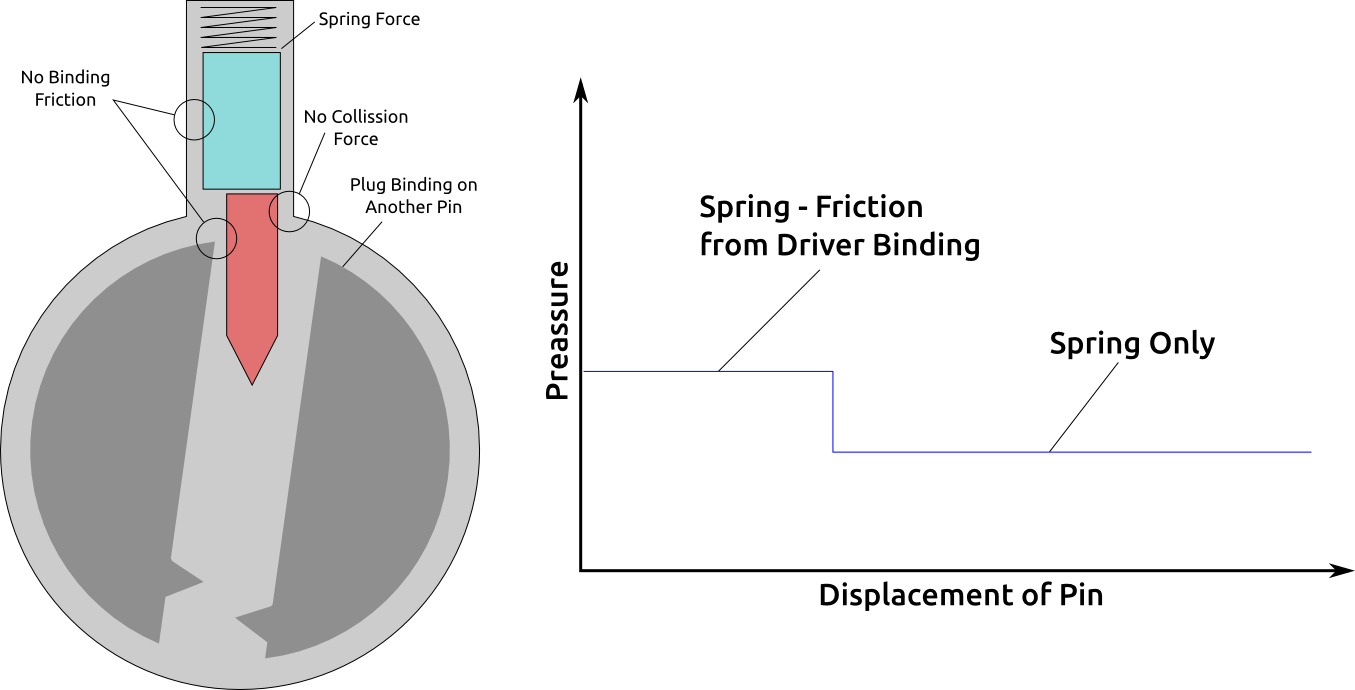
\includegraphics[scale=0.3]{figure9.3}
    \caption{Driver pin wider than key pin}
\end{figure}

\begin{figure}
    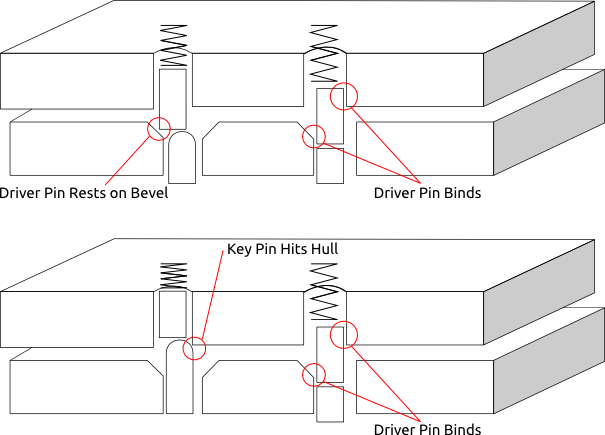
\includegraphics[width=\textwidth]{figure9.4}
    \caption{Beveled plug holes and rounded key pins}
\end{figure}

\section{Mushroom Driver Pins}
A general trick that lock makers use to make picking harder is to modify the shape of the driver pin.
The most popular shapes are mushroom, spool and serrated, see Figure 9.7.
The purpose of these shapes is to cause the pins to false set low. These drivers stop a picking technique called vibration picking (see section 9.12), but they only slightly complicate scrubbing and one-pin-at-a-time picking (see chapter 4).

If you pick a lock and the plug stops turning after a few degrees and none of the pins
can be pushed up any further, then you known that the lock has modified drivers. Basically,
the lip of the driver has caught at the sheer line. See the bottom of Figure 9.7. Mushroom
and spool drivers are often found in Russwin locks, and locks that have several spacers for
master keying.

You can identify the positions with mushroom drivers by applying a light torque and
pushing up on each pin. The pins with mushroom drivers will exhibit a tendency to bring
the plug back to the fully locked position. By pushing the key pin up you are pushing the
flat top of the key pin against the tilted bottom of the mushroom driver. This causes the
driver to straighten up which in turn causes the plug to unrotate. You can use this motion
to identify the columns that have mushroom drivers. Push those pins up to sheer line; even
if you lose some of the other pins in the process they will be easier to re-pick than the pins
with mushroom drivers. Eventually all the pins will be correctly set at the sheer line.

One way to identify all the positions with mushroom drivers is to use the flat of your pick
to push all the pins up about halfway. This should put most of the drivers in their cockable
position and you can feel for them.

To pick a lock with modified drivers, use a lighter torque and heavier pressure. You want
to error on the side of pushing the key pins too far into the hull. In fact, another way to
pick these locks is to use the flat side of your pick to push the pins up all the way, and apply
very heavy torque to hold them there. Use a scrubbing action to vibrate the key pins while
you slowly reduce the torque. Reducing the torque reduces the binding friction on the pins.
The vibration and spring force cause the key pins to slide down to the sheer line.

The key to picking locks with modified drivers is recognizing incorrectly set pins. A
mushroom driver set on its lip will not have the springy give of a correctly set driver.
Practice recognizing the difference.

\begin{figure}
    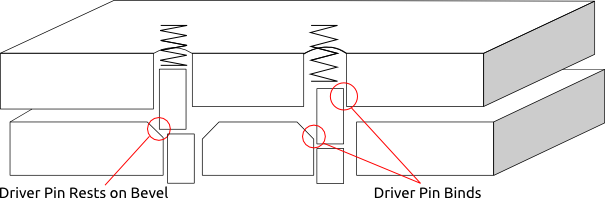
\includegraphics[width=\textwidth]{figure9.5}
    \caption{(a) Driver sets on bevel}
\end{figure}

\begin{figure}
    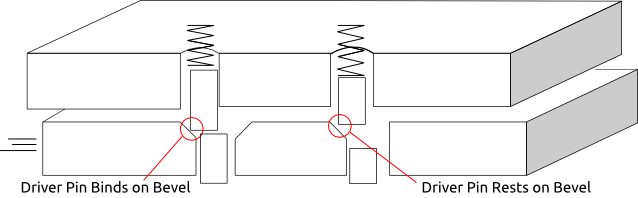
\includegraphics[width=\textwidth]{figure9.6}
    \caption{(b) Driver jams on bevel}
\end{figure}

\section{Master Keys}
Many applications require keys that open only a single lock and keys that open a group
of locks. The keys that open a single lock are called change keys and the keys that open
multiple locks are called master keys. To allow both the change key and the master key to
open the same lock, a locksmith adds an extra pin called a spacer to some of the pin columns.
See Figure 9.8. The effect of the spacer is to create two gaps in the pin column that could
be lined up with the sheer line. Usually the change key aligns the top of the spacer with the
sheer line, and the master key aligns the bottom of the spacer with the sheer line (the idea
is to prevent people from filing down a change key to get a master key). In either case the
plug is free to rotate.

In general, spacers make a lock easier to pick. They increase the number of opportunities
to set each pin, and they make it more likely that the lock can opened by setting the all the
pins at about the same height. In most cases only two or three positions will have spacers.
You can recognize a position with a spacer by the two clicks you feel when the pin is pushed
down. If the spacer has a smaller diameter than the driver and key pins, then you will feel a
wide springy region because the spacer will not bind as it passes through the sheer line. It is
more common for the spacer to be larger than the driver pin. You can recognize this by an
increase in friction when the spacer passes through the sheer line. Since the spacer is larger
than the driver pin, it will also catch better on the plug. If you push the spacer further into
the hull, you will feel a strong click when the bottom of the spacer clears the sheer line.

Thin spacers can cause serious problems. If you apply heavy torque and the plug has
beveled holes, the spacer can twist and jam at the sheer line. It is also possible for the spacer
to fall into the keyway if the plug is rotated 180 degrees. See section 9.11 for the solution to
this problem.

\begin{figure}
    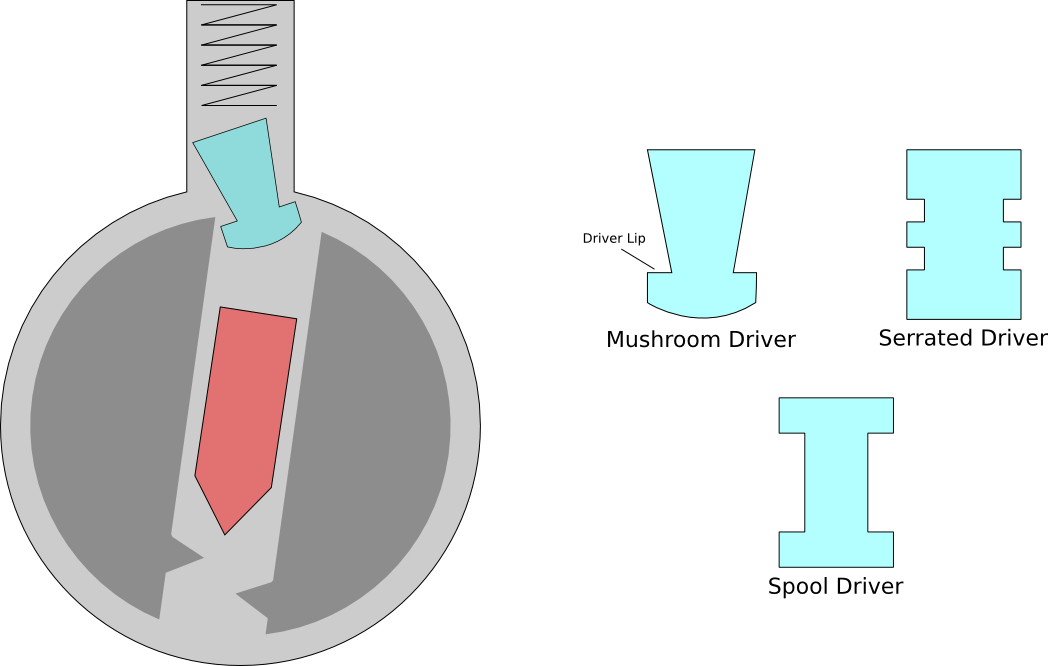
\includegraphics[width=\textwidth]{figure9.7}
    \caption{Mushroom, spool, and serrated driver pins}
\end{figure}

\begin{figure}
    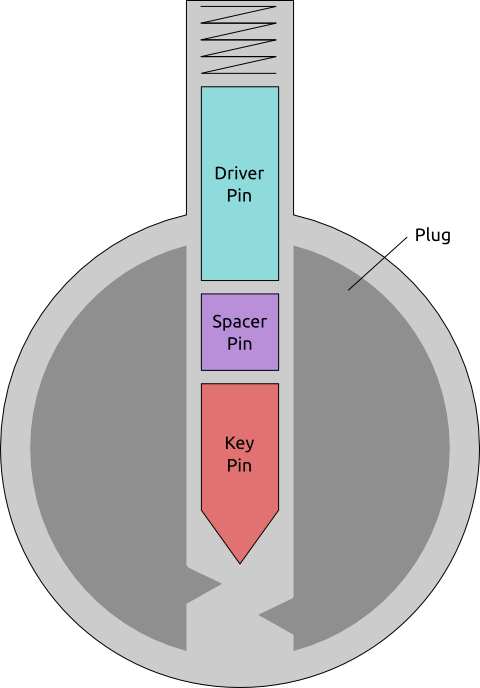
\includegraphics[scale=0.6]{figure9.8}
    \caption{Spacer pins for master keying}
\end{figure}

\section{Driver or Spacer Enters Keyway}

Figure 9.9 shows how a spacer or driver pin can enter the keyway when the plug is rotated
180 degrees. You can prevent this by placing the flat side of your pick in the bottom of the
keyway before you turn the plug too far. If a spacer or driver does enter the keyway and
prevent you from turning the plug, use the flat side of you pick to push the spacer back into
the hull. You may need to use the torque wrench to relieve any sheer force that is binding
the spacer or driver. If that doesn't work try raking over the drivers with the pointed side
of your pick. If a spacer falls into the keyway completely, the only option is to remove it. A
hook shaped piece of spring steel works well for this, though a bent paperclip will work just
as well unless the spacer becomes wedged.

\begin{figure}
    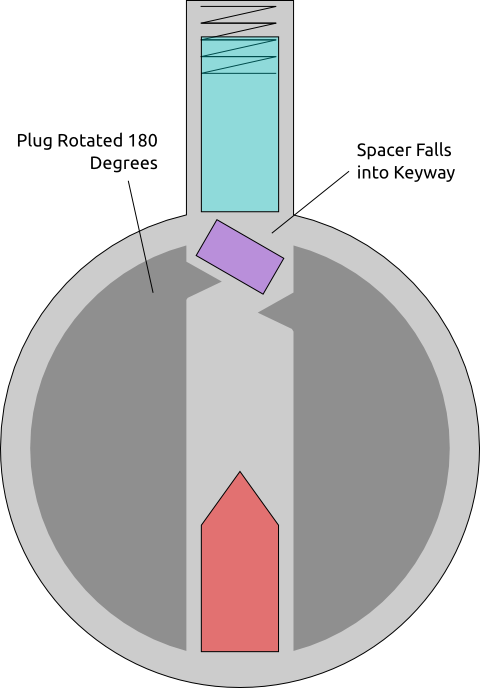
\includegraphics[scale=0.5]{figure9.9}
    \caption{Spacer or driver can enter keyway}
\end{figure}

\section{Vibration Picking}
Vibration picking works by creating a large gap between the key and driver pins. The
underlying principle is familiar to anyone who has played pool. When the queue ball strikes
another ball squarely, the queue ball stops and the other ball heads off with the same speed
and direction as the queue ball. Now imagine a device that kicks the tips of all the key pins.
The key pins would transfer their momentum to the driver pins which would fly up into the
hull. If you are applying a light torque when this happens, the plug will rotate when all the
drivers are above the sheer line.

\section{Disk Tumblers}
The inexpensive locks found on desks use metal disks instead of pins. Figure 9.10 shows the
basic workings of these locks. The disks have the same outline but differ in the placement
of the rectangular cut.

These locks are easy to pick with the right tools. Because the disks are placed close
together a half-round pick works better than a half-diamond pick (see Figure A.l). You may
also need a torque wrench with a narrower head. Use moderate to heavy torque.

\begin{figure}
    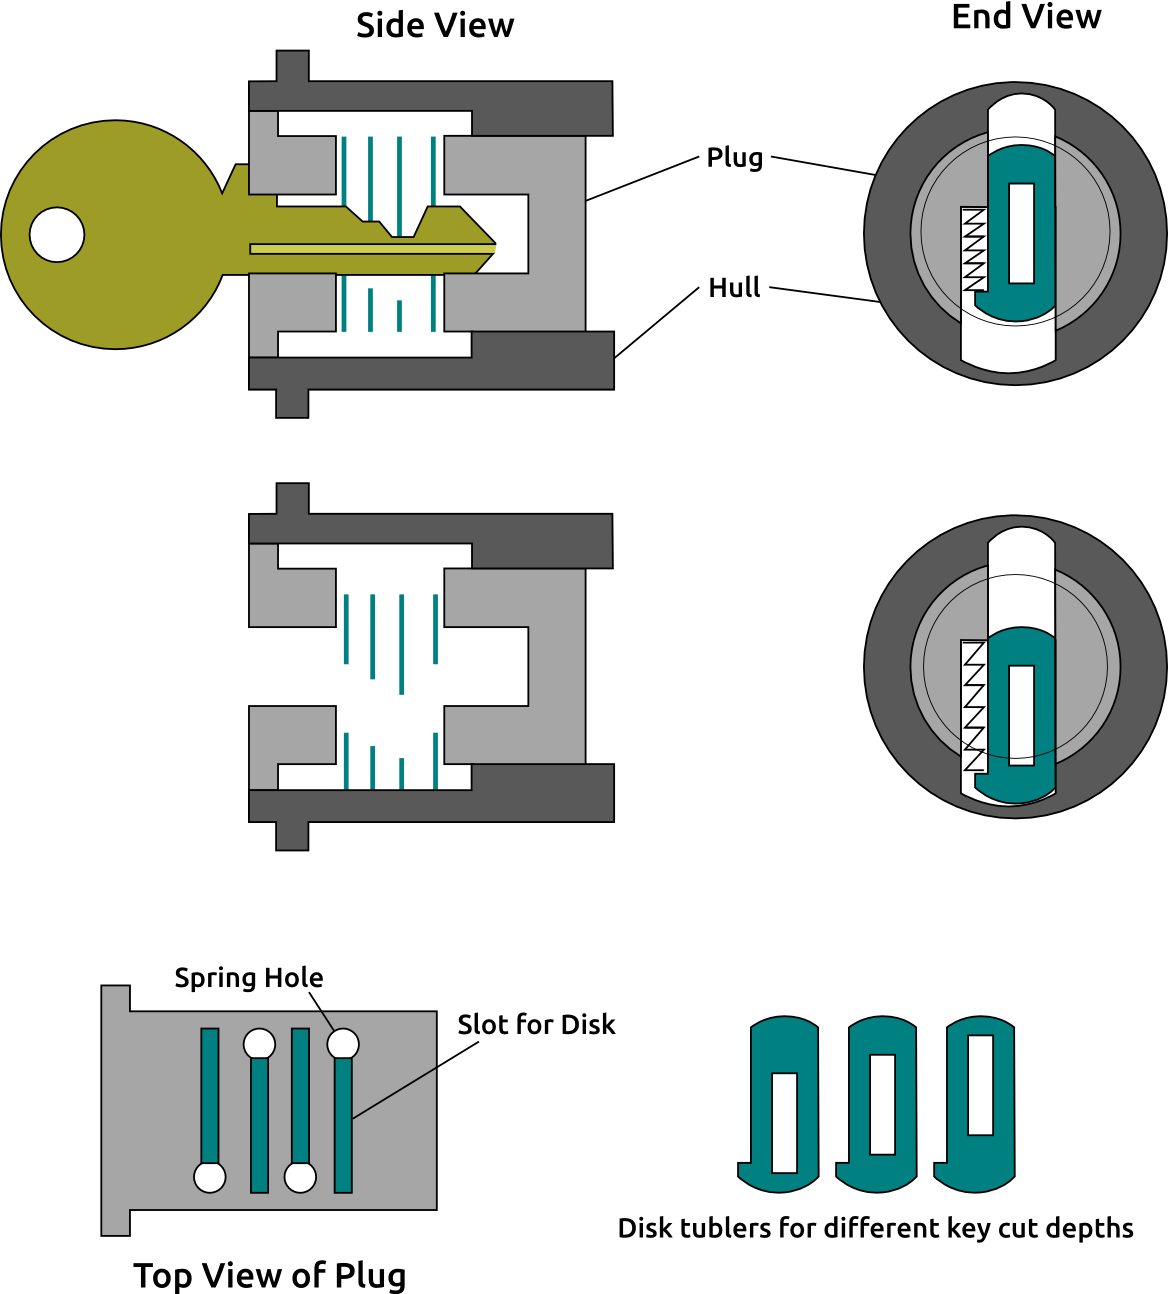
\includegraphics[scale=0.5]{figure9.10}
    \caption{Workings of a disk tumbler lock}
\end{figure}
